%!TEX root = ./thesis.tex

% \chapter{Template}\label{chapter:kapitellabel} %%%%%%%%%%%%%%%%%%%%%%%%%%%%
% \section{Test}
% \subsection{Sub Test}
% Itaque earum rerum hic tenetur a sapiente delectus, ut aut reiciendis voluptatibus maiores alias consequatur aut perferendis doloribus asperiores repellat\cite{aho:dragonbook}. See Table ~\ref{table:speedup1} and ~\ref{table:speedup1} and \ref{figure:helloworld}.

% \begin{table}[!th]
%   \renewcommand{\arraystretch}{1.3}
%   \caption{Speed-Up Table I}\label{table:speedup1}
%   \vspace{4mm} % hack
%   \centering
%     \begin{tabular}{|l||r|r|r|}
%       \hline
%       program            & basline   & algorithm 1  & alogrithm 2\\
%       \hline
%       \hline
%       {\tt simple}       &  30 sec   &  20 sec      &  18 sec     \\
%       \hline
%       {\tt hello world}  &  43 sec   &  27 sec      &  28 sec     \\
%       \hline
%     \end{tabular}
% \end{table}

% \begin{table}[!th]
%   \renewcommand{\arraystretch}{1.3}
%   \caption{Speed-Up Table II}\label{table:speedup2}
%   \vspace{4mm} % hack
%   \centering
%     \begin{tabular}{|l||r|r|r|}
%       \hline
%       program            & basline   & algorithm 1  & alogrithm 2\\
%       \hline
%       \hline
%       {\tt simple}       &  30 sec   &  20 sec      &  18 sec     \\
%       \hline
%       {\tt hello world}  &  43 sec   &  27 sec      &  28 sec     \\
%       \hline
%     \end{tabular}
% \end{table}
% Lorem ipsum dolor sit amet, consectetur adipiscing elit, sed do eiusmod tempor incididunt ut labore et dolore magna aliqua. Ut enim ad minim veniam, quis nostrud exercitation ulla hghgh hhghg mco laboris nisi ut aliquip ex ea commodo consequat. Duis aute irure dolor in reprehenderit in voluptate velit esse cillum dolore eu fugiat nulla pariatur. Excepteur sint occaecat cupidatat non proident, sunt in culpa qui officia deserunt mollit anim id est laborum

% \begin{figure}[!ht]
% \centering
% \sourcecode{main.cpp}
% \caption{Hello World Program}\label{figure:helloworld}
% \end{figure}
% Lorem ipsum dolor sit amet, consectetur adipiscing elit, sed do eiusmod tempor incididunt ut labore et dolore magna aliqua. Ut enim ad minim veniam, quis nostrud exercitation ullamco laboris nisi ut aliquip ex ea commodo consequat. Duis aute irure dolor in reprehenderit in voluptate velit esse cillum dolore eu fugiat nulla pariatur. Excepteur sint occaecat cupidatat non proident, sunt in culpa qui officia deserunt mollit anim id est laborum

% Lorem ipsum dolor sit amet, consectetur adipiscing elit, sed do eiusmod tempor incididunt ut labore et dolore magna aliqua. Ut enim ad minim veniam, quis nostrud exercitation ullamco laboris nisi ut aliquip ex ea commodo consequat. Duis aute irure dolor in reprehenderit in voluptate velit esse cillum dolore eu fugiat nulla pariatur. Excepteur sint occaecat cupidatat non proident, sunt in culpa qui officia deserunt mollit anim id est laborum~\cite{GorillaArm}

% \begin{figure}[!ht] % see https://en.wikibooks.org/wiki/LaTeX/Floats,_Figures_and_Captions for placement parameters
%   \centering
%   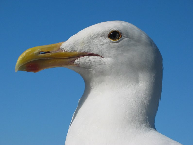
\includegraphics[width=0.5\textwidth]{images/gull.png}
%   \caption{A picture of a gull.}
% \end{figure}

% Lorem ipsum dolor sit amet, consectetur adipiscing elit, sed do eiusmod tempor incididunt ut labore et dolore magna aliqua. Ut enim ad minim veniam, quis nostrud exercitation ullamco laboris nisi ut aliquip ex ea commodo consequat. Duis aute irure dolor in reprehenderit in voluptate velit esse cillum dolore eu fugiat nulla pariatur. Excepteur sint occaecat cupidatat non proident, sunt in culpa qui officia deserunt mollit anim id est laborum

% Lorem ipsum dolor sit amet, consectetur adipiscing elit, sed do eiusmod tempor incididunt ut labore et dolore magna aliqua. Ut enim ad minim veniam, quis nostrud exercitation ullamco laboris nisi ut aliquip ex ea commodo consequat. Duis aute irure dolor in reprehenderit in voluptate velit esse cillum dolore eu fugiat nulla pariatur. Excepteur sint occaecat cupidatat non proident, sunt in culpa qui officia deserunt mollit anim id est laborum

% Lorem ipsum dolor sit amet, consectetur adipiscing elit, sed do eiusmod tempor incididunt ut labore et dolore magna aliqua. Ut enim ad minim veniam, quis nostrud exercitation ullamco laboris nisi ut aliquip ex ea commodo consequat.
% \begin{figure}[H]
%   \centering
%   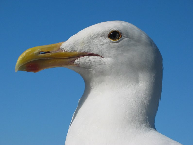
\includegraphics[width=0.5\textwidth]{images/gull.png}
%   \caption{A picture of a gull.}
% \end{figure}
% Duis aute irure dolor in reprehenderit in voluptate velit esse cillum dolore eu fugiat nulla pariatur. Excepteur sint occaecat cupidatat non proident, sunt in culpa qui officia deserunt mollit anim id est laborum

% Lorem ipsum dolor sit amet, consectetur adipiscing elit, sed do eiusmod tempor incididunt ut labore et dolore magna aliqua. Ut enim ad minim veniam, quis nostrud exercitation ullamco laboris nisi ut aliquip ex ea commodo consequat. Duis aute irure dolor in reprehenderit in voluptate velit esse cillum dolore eu fugiat nulla pariatur. Excepteur sint occaecat cupidatat non proident, sunt in culpa qui officia deserunt mollit anim id est laborum

\chapter{Einführung}\label{chapter:kapitellabel}

Zweibeiniges Gehen bietet als Fortbewegungsart durch virtuelle Umgebungen viele Vorteile gegenüber alternativen Fortbewegungsarten.[

    %TODO:Quelle
    ]
beschreibt beispielsweise, ein höheres Präsensgefühl der Nutzer:innen.[
    %TODO: Quelle

]
zeigt dass weniger Motion sickness entsteht wenn sich die Nutzer:innen durch die virtuelle Welt bewegen indem sie gehen.
[
    %TODO: quelle

]
erklärt, dass beim Gehen mehr Sinne stimuliert werden als bei künstlichen Alternativen, wie zum Beispiel der Joystick Steuerung. Tiefensensibilität (Propriozeption) und Gleichgewichtssinn (vestibuläre Wahrnehmung) signalisieren, dass er gerade wirklich geht, während diese Information bei alternativen Fortbewegungsart allein vom visuellen Sinn übermittelt wird.
Leider bring das reale gehen (real walking nach[
    %TODO: quelle

]
) auch den großen Nachteil mit sich, dass es in der Regel auf einen einzelnen Raum (den Trackingspace) beschränkt ist.

Dies entsteht zum einen, durch räumlich limitierte Erfassung (auf Englisch: tracking) der Position und Rotation des Headsets und der Controller bei einigen Technologien (zum Beispiel den Modellen der \textquote{HTC VIVE}-Produktreihe
%TODO:quelle%
), zum anderen durch die Raumgröße der meisten VR-Setups.

Zwar gibt es dazu auch Ausnahmen, ( siehe z.B.[
    %TODO: quelle microsoft studie
]
), jedoch sind diese dann mit großem Aufwand verbunden und nicht für jede Endnutzer:in umzusetzen.

\section{Redirections Techniques} %oder lieber deutsch???
%sind impossible spaces überhaupt redirected walking?
Eine Herangehensweise dieses Problem zu Umgehen sind so genannte \textquote{Redirection Techniques} (besser bekannt als Redirected Walking, diese Begriffe werden oft austauschbar verwendet (nach [
    %quelle steinicke übersicht paper

])). Dies ist ein Sammelbegriff für Techniken bei denen die Nutzer:in subtilen Manipulationen der Fortbewegungsart durch den Trackingspace navigiert wird. Dabei wird die Illusion aufrecht erhalten sie würde sich unverändert, frei bewegen. So lässt sich die Nutzer:in von den äußeren Begrenzungen des Trackingspaces fern halten, und die virtuell begehbare Fläche vergrößern.
Im folgenden werde ich nun zwei dieser Techniken genauer vorstellen.

\subsection{Rotationgains}
%TODO: quelle steinicke zusammenfassung der techniken
Rotationgains werden Kopfrotationen hinzugefügt sodass sich die virtuelle Kamera leicht schneller oder langsamer dreht als der reale
Kopf mit dem VR-Headset. Kopfrotationen lassen sich mit der Schreibweise
$$ R_{real} := (pitch_{real}, yaw_{real}, roll_{real}) $$
darstellen, wobei pitch, yaw und roll
die Eulerschen Winkel der Kopfrotation darstellen. Der Rotationgain wird dann als Quotient des virtuellen Winkels und des realen Winkels definiert also:
$$ gR := \frac{R_{virtual}}{R_{real}} $$
Für alle 3 Winkel kann ein Rotationgain angewandt werden.
Dieses Anwenden funktioniert indem der Rotationgain $gR$ mit dem Winkel der realen Kopfrotation $\alpha$ multipliziert wird also:
$$ gR * \alpha $$
Da für jeden Winkel der Kopfrotation ein Rotationgain definiert werden kann werden Rotation gains folgendermaßen dargestellt:
$$(gR_{pitch}, gR_{yaw}, gR_{roll})$$
%TODO: inline?
In der Regel wird für Redirection ein Rotationgain auf den $yaw_{real}$ Winkel der Kopfrotation angewandt.
[
    %quelle steinicke techniken
]
Durch anwenden eines rotation gains kann der virtuelle Trackingspace um den realen Trackingspace mit dem Drehpunkt der Nutzerposition herum rotiert werden.
Für den Nutzer kann so die Illusion entstehen er würde über die Grenzen des Trackingspaces hinaus schreiten können, ohne dies zu tun. (Siehe grafik)
%TODO: grafik.

\subsection{Impossible Spaces}
Um den begehbaren Bereich eines Trackingspace noch weiter zu vergrößern hat sich [
    %TODO: quelle: Suma impossible spaces q
] eine Technik ausgedacht bei der zwei oder mehr Räume in überlappenden Flächen liegen, allerdings nur einer zur Zeit angezeigt wird. Es gibt dann unterschiedliche Bedingungen, wann welcher der Räume angezeigt wird. Beispiels weise wird Raum $A$ nur angezeigt wenn die Nutzer:in den überlappenden Raum durch Tür $a$ betritt und Raum $b$, wenn sie ihn durch Tür $b$ betritt.
%TODO: grafik?
Dafür ist es also notwendig $x$ verschiedene states
%TODO: übersetzung
zu setzen sodass immer einer $x$ verschiedener Räume angezeigt wird. Des weiteren ist es Notwendig einen Bereich zu erschaffen in dem zwischen den states gewechselt werden kann, ohne dass die Nutzer:in es merkt.

\section{Generierte Level} %prozedural, oder zufällig? oder pseudozufällig?

Klassischer weise werden Level in Computerspielen und virtuellen Umgebungen von Leveldesignern designed. Dies erfordert Zeit und know-how. %TODO: formulierung
Der Arbeitsaufwand wächst (linear) mit der Größe des Levels, deshalb ist es unmöglich endlos große Level zu erschaffen. Eine alternative Levelerstellungsweise ist das so genannte \textquote{Prozedurale Generieren}(Auch \textquote{Prozedurale Synthese} genannt. Dabei wird das Level von einem Algorithmus erschaffen, und kann somit endlos große Welten erschaffen.
%verschiedene Arten von prozeduraler generiung und dazu beispiel wie minecraft, rogue etc. mit quellen.

In dem hier vorgestellten Experiment


\chapter{Verwandte Arbeiten}\label{chapter:kapitellabel}
In diesem Kapitel werden wissenschaftliche Arbeiten vorgestellt mit denen diese Arbeit zusammenhängt. Dabei werde ich zunächst auf solche Arbeiten eingehen, die sich mit dem Vergleich von Redirection Techniken zur Erweiterung des begehbaren Bereiches in virtuellen Umgebungen beschäftigen und dann auf das Thema der Level-Generierung eingehen. Zunächst stelle ich generelle Arbeiten zu dem Thema Redirection Techniken vor, danach gehe ich konkreter auf die in dieser Studie sehr im Fokus liegenden Rotationgains ein um danach die auch hier genutzten Impossible Spaces vorzustellen. Als nächstes stelle ich dem Leser noch Arbeiten vor die sich damit beschäftigt haben Level auf eine automatische Art und Weise zu generieren.

\section{Redirection Techniken}
1995 zeigte Slater et al. \cite{taking-steps}, dass Proband:innen eine höheres Präsensgefühl zeigten wenn sie die von ihm vorgestellte Technik \textquote{walking-in-place} nutzen als wenn sie per Knopfdruck durch die Welt bewegten. Hierbei handelte es sich um eine v-walking Technik bei der die Proband:innen ein eine Gehbewegung simulierten die dann digital erfasst und in Virtuell Fortbewegung umgewandelt wurde. Dieses Experiment wurde 1999 von Usoh et al. \cite{usoh-vergleich-1999} repliziert, wobei nun die Option wirklich zu gehen (\textquote{real-walking}) gegeben war. Dabei hatten die Proband:innen nochmal ein signifikant höheres Präsensgefühl als bei den beiden anderen Optionen (virtual-walking und push-button-fly).
Des weiteren zeigen Arbeiten wie \cite{benefits-real-walking} und \cite{locomotion-path-integration}, dass virtuelle Fortbewegungsarten, die anders als real-walking nicht den vestibulären Sinn und die Propriozeption stimulieren, wahrscheinlicher die sogenannte \textquote{simulator-sickness} auslösen und, dass die User:innen damit weniger effektiv navigieren.
Eine vielversprechende Art den begehbaren Bereich zu vergrößern sind Redirection Techniken. Razzaque et al. \cite{rdw-razzaque} stellte 2001 die Technik des redirected walking vor, bei der die Nutzer:innen unwissentlich durch den Trackingspace gelenkt werden, dabei aber die Illusion entsteht, sie würden sich über die Grenzen dessen hinausbewegen. Seit dem gibt es zahlreiche weitere Techniken um den selben Effekt zu erzielen oder um ihn weiterzuentwickeln. Der Ansatz die verschiedenen Manipulationseffekte als \textquote{gains} zu beschreiben findet sich bei Steinicke et al. \cite{detection-thresholds}. Dort wird untersucht wie subtil diese Manipulationen sein müssen um nicht von der Nutzer:in erkannt zu werden.
Eine Taxonomie über die verschiedenen Redirection Techniken stellte 2012 Suma et al. \cite{taxonomy} vor. Die unterschiedlichen Techniken werden in die Kategorien: \textquote{Repositioning} (Repositionierung) oder \textquote{Reorientation} (Reorientierung), \textquote{Subtle} (subtil) oder \textquote{Overt} (unverborgen), und \textquote{Discrete} (diskret) oder \textquote{Continuous} (kontinuierlich) unterteilt.

\subsection{Rotation Gains}

Bei Rotationgains handelt es such nach Sumas Taxonomie (\cite{taxonomy}) um eine kontinuierliche, subtile Reorientierungstechnik.





\chapter{Fortbewegungsarten}\label{chapter:kapitellabel}

\chapter{Implementierung}\label{chapter:kapitellabel}

\chapter{Experiment}\label{chapter:kapitellabel}
\section{Teilnehmer}\label{chapter:kapitellabel}
\section{Materialien}\label{chapter:kapitellabel}
\section{Methoden}\label{chapter:kapitellabel}
\section{Ergebnisse}\label{chapter:kapitellabel}

\chapter{Diskussion}\label{chapter:kapitellabel}

\chapter{Konklusion}\label{chapter:kapitellabel}

\chapter{Acknowledgments}\label{chapter:kapitellabel}


% keep an blank line above